\section{Realtime planlægning i \pycsp}
\label{sec:rtp-pycsp}

Da vi ønsker at introducere RTP i \pycsp er der er række forhold som vi skal tage højde for. Vi vil i dette afsnit tage udgangspunkt i de ovenstående opstillede muligheder og sammenholde dem med \pycsp. 

I \pycsp kan vi anskue processerne som begivenheder, og derved bruge skemaplanlæggeren i greenlets-versionen til at styre hvilken proces og dermed hvilken begivenhed der udføres. Vi har ikke umiddelbart informationer om hvor lang tid en proces er om at blive udført, og det vil kræve en analyse af den enkelte proces at udlede estimater for det. Vi har valgt at fokusere på selve planlægningen af processerne og ikke analyse af processerne. Dermed har vi ikke mulighed for både at benytte RM og LL algoritmerne da de begge benytter information om udførselstiden for en proces. Derved har vi EDF tilbage som mulighed, hvilket er den algoritme som vi vil implementere. En udviddelse af \pycsp til at benytte EDF er forholdsvis ligetil. Der skal laves en mulighed for at brugeren kan angive en deadline til en proces, og vi skal ved kontekstskift sikre at vi aktiverer den proces der har den førstkomne deadline. \pycsp har per definition interne afhængigheder mellem processerne i form af kommunikation over kanaler, og vi kan derfor opleve problemer med prioritetsinvertering. Den eneste metode til håndtering af prioritetsinvertering der kan bruges sammen med \pycsp er prioritetsnedarvning, da de andre metoder forudsætter prioritetsinverteringen  sker som resultat af kritiske regioner og ikke pga.  kommunikation. Vi skal derfor også implementere prioritetsnedarvning for at sikre os mod prioritetsinvertering. Endeligt skal vi håndtere overskredne deadlines.

Da vi benytter os af greenlets-versionen af \pycsp arbejder vi med en skemaplanlægger der ikke kan foretage preemptive kontekstskift. Dette kan lede til problemstillinger som det illustreret på \cref{fig:edf-nonpreemptive}. En metode til at mindske denne type problemer er at lade de enkelte processer afgive kontrollen med jævne mellemrum. Herved vil der blive foretaget en ny evaluering om hvilken proces der skal aktiveres, og hvis der processer der har en nærmere deadline som er blevet klar, aktiveres en af disse. Dette beror helt og holdent på hver at hver enkelt proces frivilligt afgiver kontrollen og gør det med jævne mellemrum når den er aktiv. Dette betyder at det er overladt til udvikleren at indsætte det på relevante steder i processens kode. 

\subsection{Prioritetsnedarvning}\label{sec:rtp-pycsp-nedarvning}
At introducere prioritetsnedarvning i \pycsp virker umiddelbart ligetil idet vi kan se de indbyrdes afhængigheder klart ud fra forbindelserne gennem kanaler. Der kan forekomme andre afhængigheder som er mindre synlige, men vi mener ikke disse vil forekomme i velskrevne CSP applikationer, og vi har derfor valgt at begrænse os til afhængigheder repræsenteret vha. kanaler. På trods af den umiddelbare simplicitet skal vi overveje hvornår, hvem og hvor længe der skal arves i forbindelse med prioritetsnedarvning.

\subsubsection*{Ændring af prioritet}
\label{sec:aendring-af-prioritet}
Vi arbejder med et dynamisk system af processer, hvor en proces, afhængig af dens tilstand, er afhængig af forskellige andre processer for at kunne arbejde videre. 
Hvis vi højner prioriteten på alle processer der er forbundet til en proces med høj prioritet vil mange af processerne der arver den høje prioritet reelt ikke kunne bidrage til udførelsen af den proces der starter med høj prioritet. Det er en bedre løsning at det kun er den eller de processer der kan sikre videre udførsel af den aktuelle proces der tildeles højere prioritet. Hvis eksempelvis en proces med høj prioritet ønsker at skrive på en kanal, skal alle processer der læser på den kanal arve den høje prioritet, men processer som ønsker at skrive til en anden kanal som processen med høj prioritet læser fra, skal ikke arve den høje prioritet. Generelt set betyder det at der kun skal udføres prioritetsnedarvning såfremt en proces venter på at kommunikere, uden der er andre processer der er klar til at indgå i den ønskede kommunikation. 

Vi har nu begrænset os til det kun er  processer der kan indgå i kommunikation over en kanal der arver en prioritet. Med any-to-any kanaler findes der dog et vilkårligt antal processer i hver kanalende, og man risikerer en prioritetsdevaluering ved at lade flere processer arve en høj prioritet. I klassisk \csp findes der modsat hertil one-to-one kanaler, hvor man er sikret at ved prioritetsnedarvning kun én proces' prioritet der bliver højnet. Forskellen kan illustreres af \autoref{fig:one-to-one-inheritance} og \cref{fig:any-to-any-inheritance}\fxwarning{tjek sidenr. er korrekt for de to figurer inden aflevering}. I \autoref{fig:one-to-one-inheritance}, bliver en proces' prioritet hævet fra fem til ti. Modtageren kan uden afbrydelser arbejde hen mod at kunne kommunikere, da afsenderen venter. I \autoref{fig:any-to-any-inheritance} bliver alle tre processers prioritet hævet til ti og de vil skulle kæmpe mod hinanden for komme frem til en tilstand hvor de ønsker at kommunikere. 

\begin{figure}
 \begin{center}
  
\includegraphics[scale=1.00]{images/one-to-one-inheritance}
\caption{Procesnetværk med en afsender og en modtager. Afsenderen har prioritet ti, mens modtageren har en initiel prioritet på fem. Modtageren  får via prioritetsnedarvning hævet sin prioritet til ti. (Højere er bedre)}
  \label{fig:one-to-one-inheritance}
  \end{center}
\end{figure}

\begin{figure}
 \begin{center}
  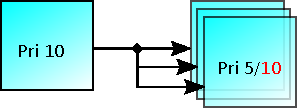
\includegraphics[scale=1.00]{images/any-to-any-inheritance}
  \caption{I dette eksempel findes der tre modtagere, som alle får hævet deres prioritet til ti.}
  \label{fig:any-to-any-inheritance}
  \end{center}
\end{figure}

 Prioritetsnedarvning i et miljø med med any-to-any kanaler har dermed en latent risiko for at medfører prioritetsdevaluering. Man kan forstille sig forskellige metoder til at eliminere eller minimere problemet f.eks ved at begrænse antallet processer der kan modtage en prioritetsnedarvning. Dette kunne gøres ved kun at lade en proces arve prioriteten,  men så skal man tage stilling til hvilken proces der skal udvælges. Dette kunne være den process der er tættets på at indgå i kommunikationen.  Udvælgelsen processer må dog bero på en analyse af den enkelte applikation og dennes aktuelle tilstand. Da vi ikke ønsker at  begynde på en analyse af  brugerens kode må vi nødvendigvis sende prioritetsnedarvningen til alle processerne på kanalen, men vil i stedet fokusere på at minimere antallet af processer der starter prioritetsnedarvningen, og den tid processerne har arvet en prioritet.

Når kommunikationen på kanalen er gennemført, befinder processens sig i en anden tilstand og er afhængig af noget andet for at komme videre i sin udførsel. 
Når det midlertidige afhængighedsforhold ophører skal processer der har arvet en prioritet miste denne. Der skal selvfølgelig tages højde for at en proces kan arve forskellige prioriteter fra forskellige andre processer, så det skal være muligt at falde tilbage til den næsthøjeste arvede prioritet, i stedet for blot at skifte tilbage til den oprindelige prioritet. 

\subsubsection*{Prioritetsnedarvning i alternation}%\code{alternations}}
Vi har som nævnt en klar kæde af afhængigheder i \pycsp men vi skal være opmærksomme på ikke at højne processers prioritet unødigt. Dette kan let være tilfældet såfremt vi ikke holder ordentligt styr på hvorfor en proces har den prioritet den har, om den er sat af udvikleren eller den er nedarvet. Man kan forestille sig en situation hvor et uddrag af et proces-neværk består af en generator-forbruger model med to generatorer og en enkelt forbruger. De to generatorer er forbundet til forbrugeren vha. en \code{alternation} og generatorerne har henholdsvis høj og lav prioritet. Eksemplet er illustreret på \cref{fig:alt-inheritance}. Forbrugeren vil i dette scenarie arve den høje prioritet fra den tilsvarende generator, men utilsigtet vil den høje prioritet også propagere fra forbrugeren til generatoren med lav prioritet. Dette er ikke hensigtsmæssigt da de to generatorer nu har lige høj prioritet og ikke det forhold som udvikleren oprindeligt har angivet. Vi kan dog indse at dette ikke bliver et problem idet vi kun udfører prioritetsnedarvning i det tilfælde at der ikke er nogen processer der er er klar til at indgå i ønsket kommunikation. I det opstillede tilfælde vil forbrugeren derfor ikke foretage yderligere prioritetsnedarvning på generatoren med lav prioritet, da generatoren med høj prioritet altid vil være klar til at skrive i denne situation. 

\begin{figure}
 \begin{center}
  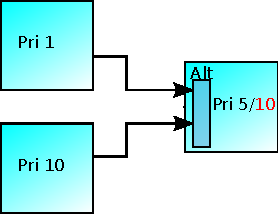
\includegraphics[scale=1.00]{images/alt-inheritance}
  \caption{Prioritetsnedarvning i \code{alternations}}
  \label{fig:alt-inheritance}
  \end{center}
\end{figure}


\subsection{Tilknytning og overskridelse af deadlines}
Som udgangspunkt skal vi kunne håndtere at en proces kan have forskellige typer deadlines. Umiddelbart giver det mening at der for hver proces tilknyttes en deadline samt hvilken type det er. Dette giver mulighed for at vi kan differentiere i måden hvorpå vi håndterer en overskreden deadline. F.eks. kan vi stoppe systemet helt i tilfælde af overskridelse af en kritisk deadline, kaste en exception ved en hard deadline og blot registrere overskridelser af soft deadlines. Uanset hvilken handling vi vælger at tilknytte til de respektive overskridelser, vil der være situationer hvor den valgte handling ikke er optimal. Vi har derfor valgt en anden løsning hvor en proces blot kaster en exception hvis den overskrider en deadline. Dette overflødiggør at der tilknyttes en specifik type deadline til en proces, da håndteringen af den kastede exception overgives til udvikleren. Det er herved op til den nekelte udvikler at definere hvad der skal ske i i hver enkelt proces såfremt den oplever en overskreden deadline. Dette giver den største frihed til at tilpasse håndteringen til den enkelte proces og applikation. 

\subsection{Udvælgelse i \code{alternations}}
Som  beskrevet af \citeauthor{Burns1990}, opstår der en konflikt ved brugen af  prioriterede valg. ifh. til prioriteter på processer \cite{Burns1990}. De beskriver en kodestump som angivet i \cref{lst:pri-select}, hvor processernes prioritet er angivet som Pri1 og Pri2, og hvilken proces der udvælges afhænger af processernes indbyrdes forhold som angivet i \cref{tab:prioritizedSelect}.


\begin{lstlisting}[firstnumber=1 ,float=hbtp, label=lst:pri-select, caption={(priority) select. Eksemplet er kopieret fra \cite{Burns1990}}]
(priority) select
   A1 -- Process P1
 or
   A2 -- Process P2
 end select
\end{lstlisting}

\begin{table}[htbp]
	\centering
	\begin{tabular}{lccc}
       	\toprule
        &Pri1 > Pri2 & Pri1 = Pri2 & Pri1 < Pri2\\
        \midrule
          	select          & A1 & Arbitrary    & A2 \\
		    priority select & A1 & A1           & ? \\    
        \bottomrule
        \end{tabular}
    \caption[]{Konflikten ved brug af prioriteret valg og procesprioriteter. Eksemplet er kopieret fra \cite[160]{Burns1990}}\\
    \label{tab:prioritizedSelect}
\end{table}

I \pycsp findes kun et prioriteret valg, og dermed kan vi se bort fra første række af \cref{tab:prioritizedSelect}, og konstatere at vi introducerer  en konflikt med introduktionen af prioriteter. For \citeauthor{Burns1990} er løsningen ``orthogonal solutions'', der  tager hånd om begge typer af prioriteter. De ønsker overordnet set to typer udvælgelsesmetoder, Weak- og Strong Select. Weak select sorterer primært ifh. til processernes prioritet og sekundært efter det prioriterede valg. Strong select udvælger udelukkende processer efter det prioriterede valg. De forestiller sig at weak select skal bruges som den primære metode, men i hjørnetilfælde skal en programmør have mulighed for at tvinge et prioriteret valg igennem.

Vi ønsker at foretage udvælgelse i \code{alternations} udføres som weak select. Dvs at først skal der kigges der på om alternation kan vælge en guard umiddelbart. Hvis der er minimum en guard klar foretages der et prioriteret valg baseret på først processernes prioritet, og hvis flere processer har samme prioritet  foretages det prioriterede valg. Er ingen guards klar bør processen vente i dens alternation, og vælge den første guard der bliver klar, uden at skele til dens prioritet.

I artiklen fra \citeauthor{Burns1990} udvælger man en proces blandt flere mulige, mens en \code{alternation} udvælger en kanal der i \pycsp er af typen any-to-any. Dette medfører at man ikke  foretager et valg mellem processer, men foretager et valg mellem kanaler, som processen kommunikerer med. For at foretage en weak selection i vores \code{alternation}, skal man derfor kunne finde prioriteten for kanalerne. Dette skaber derfor et behov for at kunne tilknytte en prioritet til hver kanal, baseret på hvilke processer der er tilknyttet kanalen. 
\phantomsection
\label{misc:kanal-prioritet}



